% This is "sig-alternate.tex" V1.3 OCTOBER 2002
% This file should be compiled with V1.6 of "sig-alternate.cls" OCTOBER 2002
%
% This example file demonstrates the use of the 'sig-alternate.cls'
% V1.6 LaTeX2e document class file. It is for those submitting
% articles to ACM Conference Proceedings WHO DO NOT WISH TO
% STRICTLY ADHERE TO THE SIGS (PUBS-BOARD-ENDORSED) STYLE.
% The 'sig-alternate.cls' file will produce a similar-looking,
% albeit, 'tighter' paper resulting in, invariably, fewer pages.
%
% ----------------------------------------------------------------------------------------------------------------
% This .tex file (and associated .cls V1.6) produces:
%       1) The Permission Statement
%       2) The Conference (location) Info information
%       3) The Copyright Line with ACM data
%       4) Page numbers
%
% as against the acm_proc_article-sp.cls file which
% DOES NOT produce 1) thru' 3) above.
%
% Using 'sig-alternate.cls' you have control, however, from within
% the source .tex file, over both the CopyrightYear
% (defaulted to 2002) and the ACM Copyright Data
% (defaulted to X-XXXXX-XX-X/XX/XX).
% e.g.
% \CopyrightYear{2003} will cause 2002 to appear in the copyright line.
% \crdata{0-12345-67-8/90/12} will cause 0-12345-67-8/90/12 to appear in the copyright line.
%
% ---------------------------------------------------------------------------------------------------------------
% This .tex source is an example which *does* use
% the .bib file (from which the .bbl file % is produced).
% REMEMBER HOWEVER: After having produced the .bbl file,
% and prior to final submission, you *NEED* to 'insert'
% your .bbl file into your source .tex file so as to provide
% ONE 'self-contained' source file.
%
% ================= IF YOU HAVE QUESTIONS =======================
% Questions regarding the SIGS styles, SIGS policies and
% procedures, Conferences etc. should be sent to
% Adrienne Griscti (griscti@acm.org)
%
% Technical questions _only_ to
% Gerald Murray (murray@acm.org)
% ===============================================================
%
% For tracking purposes - this is V1.3 - OCTOBER 2002

\documentclass{sig-alternate-sigmod07}

\usepackage{tablefootnote}
\usepackage{hyperref}
\usepackage{cleveref}
\usepackage{enumitem}

\begin{document}
%
% --- Author Metadata here ---
%\conferenceinfo{ACM SIGMOD}{'07 Beijing, China}
%\CopyrightYear{2014} % Allows default copyright year (2000) to be over-ridden - IF NEED BE.
%\crdata{0-12345-67-8/90/01}  % Allows default copyright data (0-89791-88-6/97/05) to be over-ridden - IF NEED BE.
% --- End of Author Metadata ---
\makeatletter
\def\@copyrightspace{\relax}
\makeatother
\title{Detecting short-term anomalies in gas consumption using ARIMA and Robust Artificial Neural Networks}
%
% You need the command \numberofauthors to handle the "boxing"
% and alignment of the authors under the title, and to add
% a section for authors number 4 through n.
%
\numberofauthors{2}
\author{
% You can go ahead and credit any number of authors here,
% e.g. one 'row of three' or two rows (consisting of one row of three
% and a second row of one, two or three).
%
% The command \alignauthor (no curly braces needed) should
% precede each author name, affiliation/snail-mail address and
% e-mail address. Additionally, tag each line of
% affiliation/address with \affaddr, and tag the
% e-mail address with \email.
%
% 1st. author
\alignauthor
Marco De Nadai\\
       \affaddr{Universita' degli studi di Trento}\\
      \affaddr{Master's student}\\
       \email{me@marcodena.it}
% 2nd. author
\alignauthor
Maarten van Someren\\ 
       \affaddr{Universiteit van Amsterdam}\\
       \affaddr{Science Park 107}\\
       \affaddr{Amsterdam, The Netherlands}\\
       \email{m.w.vanSomeren@uva.nl}
}
\maketitle
\begin{abstract}

The focus of this paper is on predicting and finding anomalies on gas consumption that can successively be reported to the building managers who can identify wasteful apparatus and fix them.  Even if predicting future consumption is very useful, the existing approaches separate it from the outlier detection task, typically identifying them with the Gaussian error theory. Moreover, previous examples of outliers (or cleaned data) are usually required.

In this work a 2-phase system is presented, where the first one forecasts the short-term (hourly) gas consumption, where the second phase detects outliers on the base of deviations from expected (forecast) value. Outliers are detected without possessing previously labelled examples, thanks to a very precise forecast with a RMSE error between $8$ $m^3$ and $2.5$ $m^3$. 

\end{abstract}

\keywords{Energy forecasting, Time series, Robust Artificial neural networks, ARIMA models, anomaly detection, outlier detection, gas consumption prediction, energy forecast}

\section{Introduction}

Energy consumption in buildings is one of the fastest growing sectors. Approximately $41\%$ of the total energy in Europe is consumed by buildings (households and services) \cite{Eurostat2013}. Studies and states' directives about minimizing energy consumption and using renewable energy steadily increased with the reduction of fossil fuels, the border frictions with eastern countries like Russia, and the increase of various environmental problems. Under those circumstances, the European union, with a recent directive \cite{Directive2009}, has set the target to raise EU energy consumption produced from renewable resources to $20\%$, to reduce by $20\%$ the EU greenhouse gas emissions and to improve by $20\%$ the EU's energy efficiency. This means investments to re-qualify old buildings, new energy regulations and diagnosis, but also new efficiency systems for appliances.

Forecasting energy demands has become one of the major research field in the energy departments because it helps gas utilities, but also industries and families. Gas utilities buy gas from pipeline companies on a daily bases, consequently they need to know the needs in advance to be competitive. Similarly, Companies and families have the aim of reducing the energy consumption and increase efficiency. \\
Lately, big companies like Google have shown their interest in this new market, developing thermostats which automatically control the house climate basing the decisions on users' schedule. Nest, a company acquired by Google, declared that thanks to its automatically learning thermostat, customers saved 11.3\% of AC-related energy usage without compromising comfort \cite{GoogleNest2}. Learning people behaviour can save a lot of money but system anomalies still raise and spoil the saving effort. It is showed \cite{katipamula2005review, wu2011cross} that commercial buildings consume from $15\%$ to $30\%$ more energy than necessary due to poorly maintained, degraded, and improperly controlled equipment. These anomalies can become easy fixable problems with a reliable fault detection and diagnosis (FDD) system. 

Gas consumption is very irregular and not easily predictable with classic methods. The outlier detection system presented is based on predictions made by a hybrid ARIMA-ANN which can model linear and non-linear behaviour of the data with very reliable results. Outliers are identified on the basis of deviations from forecast value. Thanks to this system days/hours with abnormally consumption can be reported to the building manager, who can further analyse and fix the HVAC system minimizing energy waste caused by the outliers.



%\label{sec:background} trovare referenze

\subsection{What is an outlier}
An outlier (or anomaly) by definition \cite{hawkins1980identification} \emph{is an observation which deviates significantly from other observations so that it creates suspicion that it was created by different dynamics}. Despite this general definition, the more appropriate way of defining outliers is highly application-dependent, because even same scenarios may require different determinations of outliers. \\
In this paper, outliers are very closely related to the time-series forecasting problem, since outliers are declared on the basis of deviations from expected (forecast) value. Outliers can have distinct main reasons: 
\begin{itemize}
\itemsep0em
  \item Defective system (e.g. a defective heater in a room).
  \item Bad human behaviour (e.g. people who leave open the window in a room while the system is trying to heat it).
  \item Defective monitoring system, where the system monitors different values from the real one, due to a malfunction, computing process errors or a recording negligence. 
\end{itemize}
Another important aspect to consider is the nature of an anomaly. Anomalies can be classified in three categories \cite{chandola2009anomaly}:\begin{description}[font=\normalfont\itshape,leftmargin=1pc]
\itemsep0em
  \item[Point Anomalies] If an individual data-point is considered anomalous with respect to the rest of the data.
  \item[Contextual Anomalies] If a data-point is anomalous in a specific context, but not otherwise. For example in Holland 35 degrees of temperature might be normal during summer but not during the winter.
  \item[Collective Anomalies] If a group of points is anomalous with respect to the entire data set. Collective Anomalies firstly appear at a point affecting the values immediately next to it. After a while, this effect dies out, leaving the time-series to its normal behaviour.
\end{description}

\begin{figure}[h!]
\centering
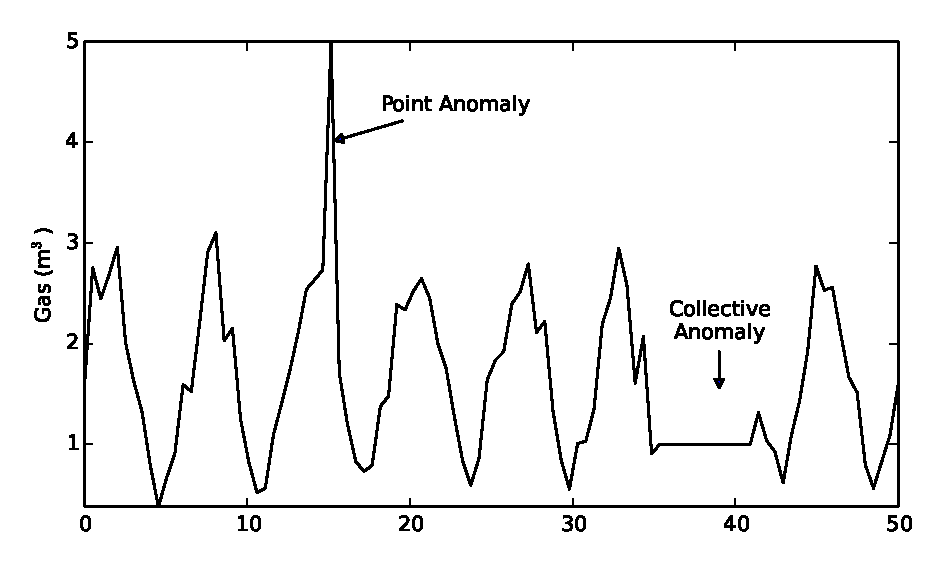
\epsfig{file=images/outlierTypes.eps, width=\columnwidth}
\caption{Different types of outliers}
\label{fig:outlierTypes}
\end{figure}


\subsection{Organization}

This paper is organized as follows. In \cref{sec:related} the major related works are explained and divided in \emph{supervised}, \emph{semi-supervised} and \emph{unsupervised} methods. In \cref{sec:proposedSolution} the solution proposed in this work is presented, describing also the possessed experimental data. Since this work uses Artificial Neural Networks and Auto-regressive methods, in the same section these are briefly explained, along with the gas forecaster. Finally, in \cref{sec:outlierDetection} the outlier detection procedure is explained. In \cref{sec:experimental} the system is completely evaluated. \cref{sec:future} presents some future ideas for the readers, based on techniques that the author didn't have the time to apply. Finally, in \cref{sec:conclusion} the conclusions are presented.


\section{Related work}
\label{sec:related}
Outlier detection system finds extensive use in a wide variety of applications such as fraud detection for credit cards, intrusion detection for cyber-security, performance analysis and fault detection in firms. Outlier detection can be \emph{supervised}, \emph{semi-supervised}, \emph{unsupervised} and since the anomaly definition is highly application dependent, in this section only the energy consumption field methods will be reviewed.


\subsection{Supervised anomaly detection}
Techniques trained in supervised mode assume the presence of labelled training data, indicating previously known examples of anomalies. There are many algorithms in this category, but all of them rely on the classification of the points in outliers or normal data. To cite some of them, in \cite{house1999classification} ANNs and Nearest neighbour classifiers are compared, while a Bayes classifier is used for fault detection. In \cite{hippert2001neural} over 20 papers of ANN classifiers were compared.


\subsection{Semi-supervised anomaly detection}
Semi-supervised models are characterized by having a training set where there are only examples for normal data. There are no so many examples of this category in the energy field. In \cite{fujimaki2005approach} this model is applied for spacecrafts fault detection. 


\subsection{Unsupervised anomaly detection}
\label{sec:unsupervised}
Unsupervised methods have no training data nor anomalies labelling. Typically most of the unsupervised outlier mechanisms use a measure of \emph{outlierness} of a data point, such as sparsity of underlying region, nearest neighbour distance or the fit to underlying distribution \cite{aggarwal2013outlier}. In these cases a data-point is unusual due to one or more variables rather than a specific one (like in the supervised methods). Literature (in the energy field) is usually based on the \emph{Gaussian error} theory. This suppose that the measurement follows the normal distribution, and outliers are the points falling outside three times the variance. One example above all is \cite{ferdowsi2013neural}, who uses and improves this method to identify outliers with a rolling median window.
Unsupervised methods are usually based clustering, where an algorithm tries to find similarities between points/trends and cluster them into groups, calculating the distance between them. A cluster is considered good when the intra-cluster distance is minimized and the intra-cluster distance is maximized. Popular methods in this group are $k$-means, one-class SVM and self-organizing maps. For example in \cite{khan2013fault} some clustering methods, like CART, $k$-means and DBScan, were applied to detect outliers in the office lighting energy consumption. The author showed different techniques applied along with the Generalized Extreme Studentized Deviate (GESD) and listed some irregularities found. He also stated that clustering methods were not able to detect faults strongly related to time variable. 

%da rimpinzare





\section{Proposed solution}
\label{sec:proposedSolution} 

The available dataset does not indicate if any instance is \emph{normal} or \emph{anomalous}, and labelling the dataset would be prohibitively expensive. For this reason an unsupervised method (\cref{sec:unsupervised}) needs to be applied. Clustering methods are very difficult to be applied in time-series (\cref{eq:timeseries}) data with decent results. The solution would be to apply a Gaussian error method, instead this project wants to be more exhaustive, and develop a new method which also provide a energy use forecast, useful for future building plans. In this work outliers are declared on the basis of deviations from expected (forecast) value.

A time-series is a sequence of data-points typically measured at successive points of a uniform time interval $t$.
\begin{equation}\label{eq:timeseries}\left\{x(t_0), x(t_1), \ldots x(t_i), x(t_{i+1}) \ldots \right\}\end{equation}
where $x$ is the value and $t$ the time. Time-series forecasting is about predicting future values given past data (\cref{eq:forecast}). 
\begin{equation}\label{eq:forecast}\hat{x}(t+s) = f\left(x(t), x(t-1) \ldots \right) \end{equation}
where $s$ is the step size. A \emph{multivariate} time-series is a $(n\times1)$ vector of $n$ time-series variables.

It can be seen that in academic and industry research, linear regression-based systems represent the standard ``de facto" of energy forecasting. These techniques are usually applied to electric consumption, which is much more easily predictable than the gas one. Moreover, they have been applied in short-term forecast, since Auto-regressive methods are potentially useless in long ahead data-points. In recent works auto/linear regressive methods were also combined weather forecast data with energy use, but this relationship is clearly non-linear \cite{hippert2001neural}. Consequently, even if some papers have acceptable results with measured datasets, these systems cannot adequately capture the relationship in all the situations and data.

Since ANNs are the state of the art technique of many machine learning problems where there are complex non-linear hypothesis, the proposed solution is based on them. Reviews of ANNs based forecasting system have concluded that they are promising but ``a significant portion of the ANN research in forecasting and prediction, lacks validity". Much work (as this one) needs to be done before they are accepted as forecasters. 

Zhang et al \cite{zhang1998forecasting} stated that ANN models really have advantages in dealing with a large amount of historical load data with non-linear characteristic, but they neglected the linear relations including the data. For this reason a hybrid approach is proposed, where the ANN is helped in linear forecasting by the popular method ARIMA (auto-regressive integrated moving averages), commonly known as the Box–Jenkins approach. 



\subsection{Experimental data}
The energy consumption datasets used were collected by Ebatech in various buildings of the Hogeschool van Amsterdam and provided by Universiteit van Amsterdam. The buildings are located in Amsterdam, the capital city of The Netherlands. This city has a maritime climate similar to England, strongly influenced by the North Sea. Winters are fairly cold and summers are rarely hot for the European standards. Amsterdam is characterized by the common presence of rain and wind and the weather conditions vary frequently.\\
Ebatech collected different features in each building, with different granularity. This project used three buildings where the features overlapped (see \cref{tab:dataset}). All these buildings were heated only by gas, which was used only for this purpose.

The weather data was collected by KNMI\footnote{Koninklijk Nederlands Meteorologisch Instituut http://www.knmi.nl} in Schipol, the Amsterdam airport 16 km far from the tested buildings. The dataset, findable in their website, consists in over 21 variables hourly collected. The proposed solution only uses few of them, as explained in the \cref{sec:predictor}, and the measured weather conditions at time $t$ are used at time $t-1$ as simulated forecast conditions. It is necessary to note that this will introduce an error in the final model, due to the effect of the weather forecast uncertainty \cite{douglas1998impacts, ranaweera1996effect}. Another error is caused by using the conditions collected in a different location from the buildings positions.

\begin{table}
\centering
\label{tab:dataset}
\begin{tabular}{|c|c|l|} \hline
Building name&Date interval&Number of rows\\ \hline\hline
HvA 740 - NTH & 01/2008 - 03/2014 & $54.725$\\ \hline
Hva 761 - KMH & 01/2009 - 09/2013 & $40.407$\\ \hline
Hva 882 - WBW& 01/2008 - 03/2014 & $54.647$\\ \hline
\end{tabular}
\caption{Buildings used.}
\end{table}



\subsubsection{Data analysis}
\label{sec:dataAnalysis}

The energy consumption dataset covers a very large period ranging more than 5 years, allowing to see similar patterns even with different yearly/seasonal behaviour (one year could be different from another one for external factors like weather or building use). The dataset is very rich (with more than 50 variables) but also sparse because the monitored variables are not the same in all the buildings.

The gas consumption data is highly seasonal: daily and weekly cycles are quite perceptible, as it can be seen from \cref{fig:monthlyTGas} and \cref{fig:dailyBehaviour}. From the latter the weekly behaviour is clear: the last two days of the week (Saturday and Sunday) are completely different from the others. Moreover Monday seems a bit different from the rest of the days. The system reveals us that after a couple of hours, it decreases the consumption again. Furthermore, around 4:00-5:00 AM the system seems to react turning on the heating system, where in the previous hours of the night it seems only keeping a minimum temperature. 

\cref{fig:monthlyTGas} shows that the temperature has a clear daily/hourly relation with the gas consumption, while in \cref{fig:monthlyGasElectr} the electric consumption is shown to be very smoothed and more regular than the gas one.


\begin{figure}[h!]
\centering
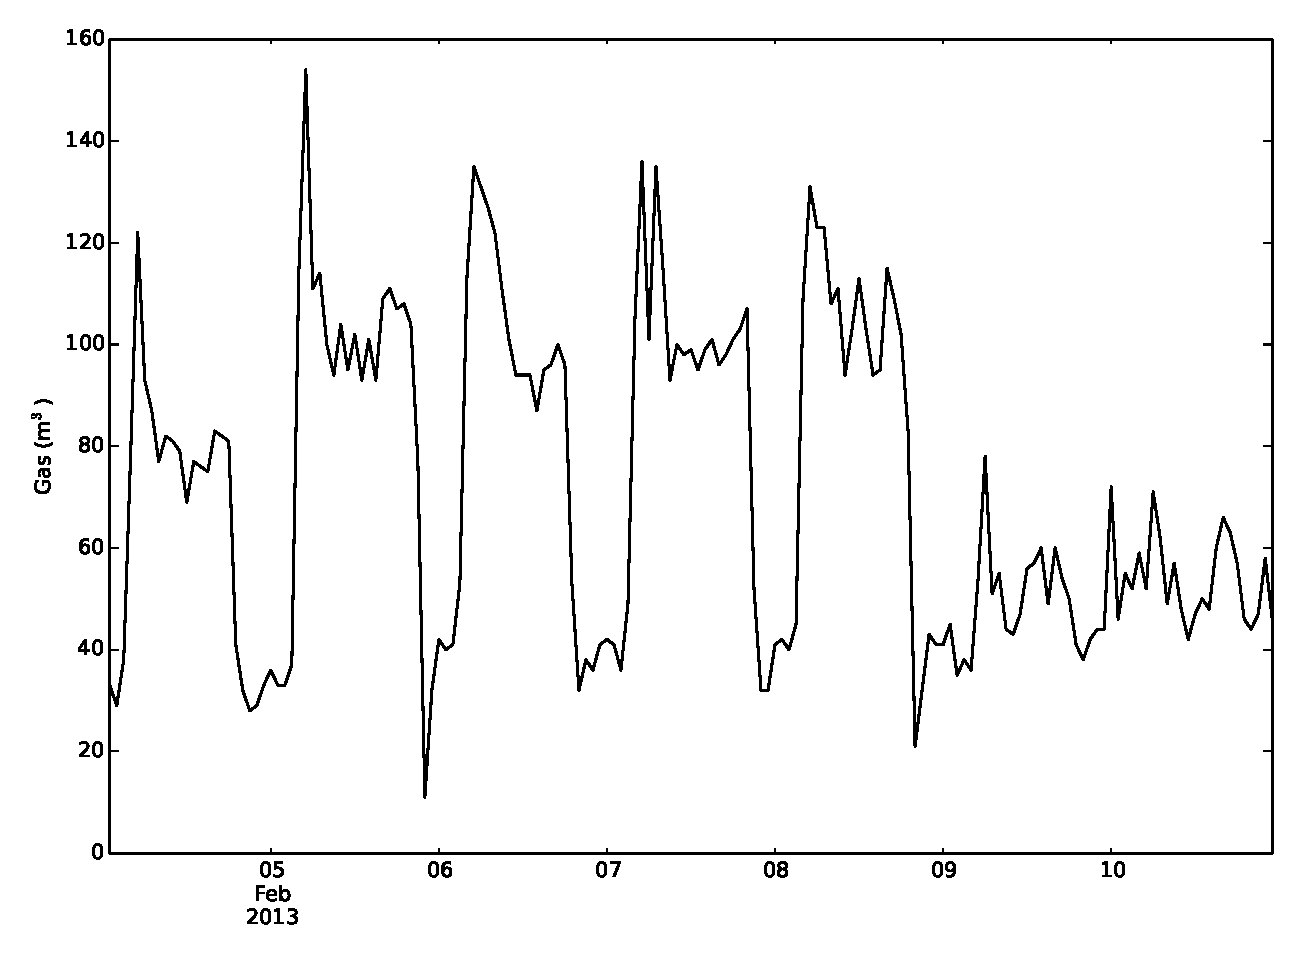
\epsfig{file=images/dailyBehaviour.eps, width=\columnwidth}
\caption{Typical weekly and daily gas consumption behaviour in building 740-NTH. The weekly pattern can be noticed by observing that the last two days of the week (Saturday and Sunday) have a completely different shape than the others. During the week, the daily behaviour is very similar, with one peak around 4:00-5:00 AM.}
\label{fig:dailyBehaviour}
\end{figure}

\begin{figure}[h!]
\centering
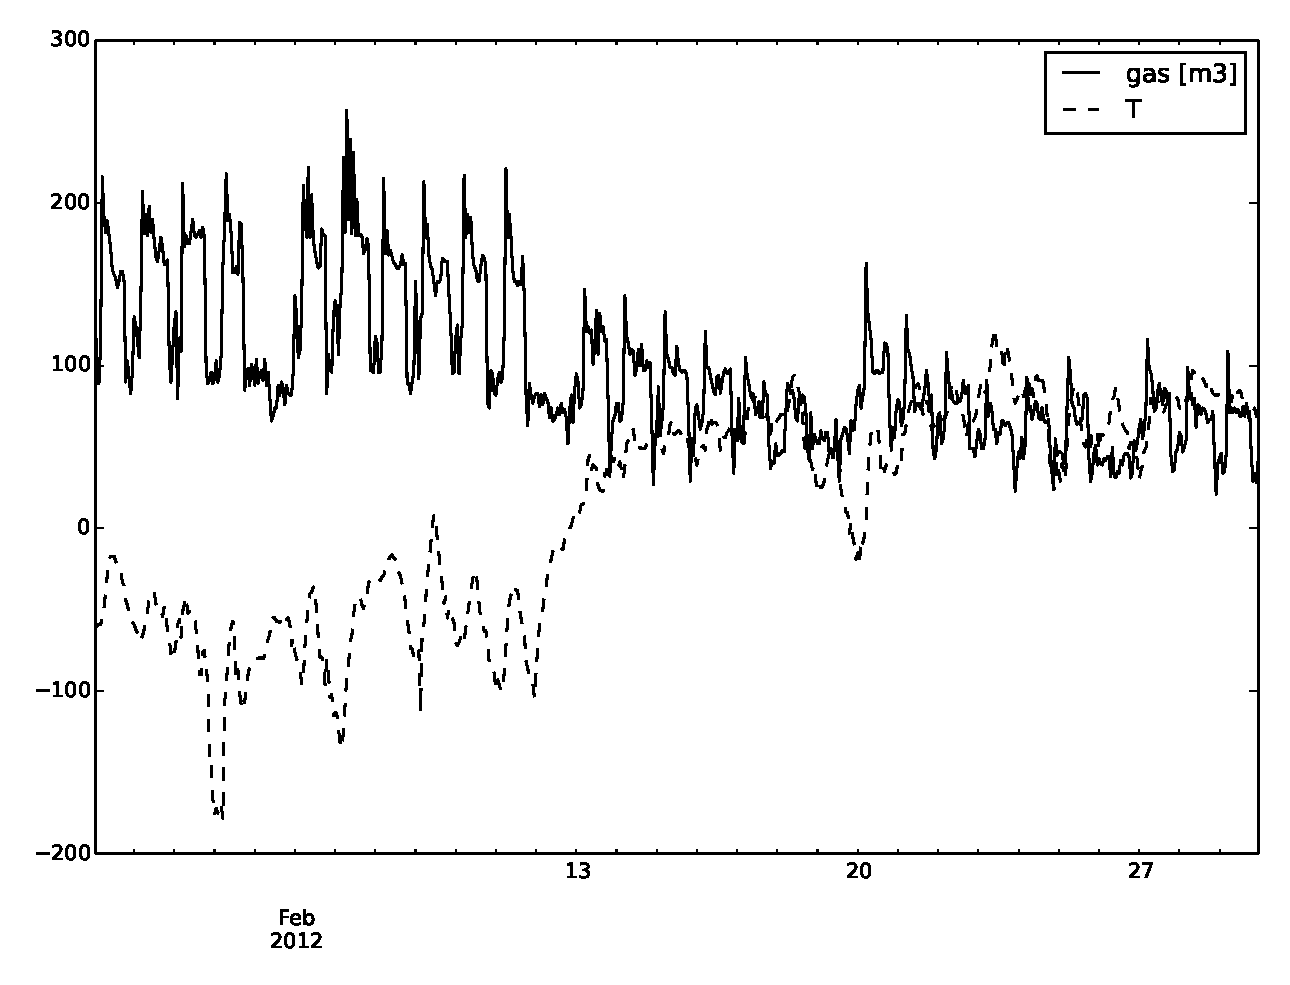
\epsfig{file=images/monthlyTGas.eps, width=\columnwidth}
\caption{Typical monthly gas consumption behaviour in building 740-NTH and its relation with the temperature in building 740-NTH.}
\label{fig:monthlyTGas}
\end{figure}

\begin{figure}[h!]
\centering
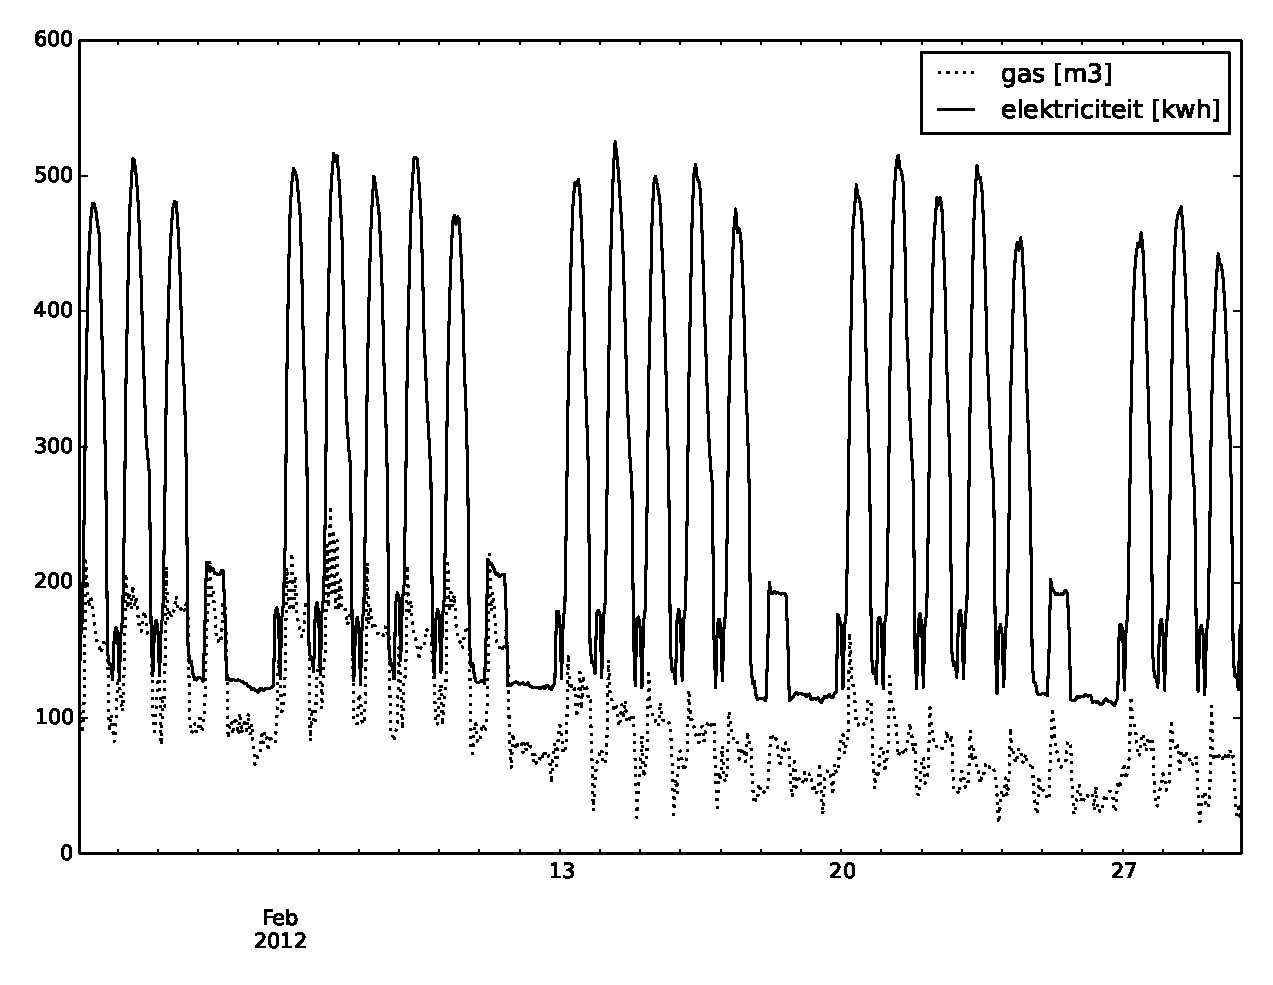
\epsfig{file=images/monthlyGasElectr.eps, width=\columnwidth}
\caption{Relation between electric and gas consumption in building 740-NTH}
\label{fig:monthlyGasElectr}
\end{figure}



\subsubsection{Data preparation}
\label{sec:cleaning}
The data presented some irregularities like repeated and missing data-points. Repeated data-points were deleted, while missing data-points were reconstructed by linear interpolation because they could cause problems to ARIMA. Cubic and spline interpolation were also considered but the performance was heavily affected by these methods.
%\vfill


\subsection{Background}


\subsubsection{Artificial Neural Networks}
Artificial Neural Networks (ANNs) were originally developed to mimic the brain functionality. The complexity of a brain neuron is abstracted by artificial neurons, also called units. These consist of \emph{weighted inputs} computed by a mathematical function which determines the \emph{activation} of a neuron. The \emph{output} is the result of this function. Neuron activations are usually represented with linear, hyperbolic tangent or sigmoid function. Recent findings argued that Rectifier units seems to be more biologically plausible \cite{glorot2011deep}.

The most famous architecture is the one showed in \cref{fig:ANN}. Neurons are usually organized in layers, where the layer between input and output is called \emph{hidden}. Neurons are usually fully connected with the neurons of the next layer. Learning is done by the Stochastic Gradient Descent (SGD) algorithm, which tries to find the best weight configuration to optimize the output (reducing a cost/error function). It is usually combined with the \emph{Backpropagation} algorithm, which back-propagates the output error to the inner levels.

More information about ANNs can be found in \cite{bishop2006pattern}.

\begin{figure}[h!]
\centering
\epsfig{file=images/NN2.eps, width=\columnwidth}
\caption{ANN with \emph{Backpropagation}, 5 inputs, 3 hidden neuron in the hidden layer, and one output (in this paper, the gas consumption value).}
\label{fig:ANN}
\end{figure}


\subsubsection{Auto-regressive models}
Let $X_1, X_2, \ldots X_t$ be the values in an univariate time-series. In the \emph{Auto-Regressive Moving Average} (ARMA) model, the value of $X_t$ is defined in terms of the values in the last windows of length $p$ and $q$ moving average terms.
\begin{displaymath}X_t =  \sum_{i=1}^p \varphi_i X_{t-i} + \sum_{i=1}^q \theta_i \varepsilon_{t-i} + c + \varepsilon_t.\end{displaymath}
The left-hand part is called auto-regressive part, because it depends on the previous (lagged) values $X_{t-1}, X_{t-2}, \ldots X_{t-p}$, the right-hand part is called moving average because the error at time $t$ is the linear combination of the previous errors $\varepsilon_{t-1}, \varepsilon_{t-2}, \ldots, \varepsilon_{t-q}$. \\
These methods are applied to \emph{stationary} time-series, so called when the mean, variance and autocorrelation structure do not change over time. However many time-series have seasonal effects or trends. In particular, random walks,
which characterise many types of series, are non-stationary. Differencing the data-points can often transform a non-stationary time-series into a \emph{stationary} one. Based on the Box-Jenkins models of the $1970s$, ARIMA models differentiate series with deterministic trends if necessary, then applies an ARMA model. ARIMA models are usually mentioned as ARIMA(p, d, q), to show the ARMA parameters and the $d$ order of difference. ARIMA models are also capable of modelling a wide range of seasonal data. 
\begin{displaymath}
\operatorname{ARIMA}(p,d,q) (P,D,Q)_m
\end{displaymath}
where $m$ is the number of periods per season. The upper-case notation $(P,D,Q)$ is used for the seasonal parts of the model, and the lower-case notation for the non-seasonal parts of the model.

The choice of the parameters $p$, $d$, $q$ is highly application dependent and it relies on theory that is beyond the scope of this paper. More information can be found in \cite{rousseeuw2005robust}.


\subsection{Artificial Neural Network forecast}
\label{sec:predictor}
Since \cref{sec:related} is focused on outliers detection works, the next subsection will try to review energy consumption forecast. After this, the features and the ANN architecture are described.


\subsubsection{Related work}
Gas forecasting is divided in three macro categories and each of them have their own techniques: short-term, medium-term and long-term forecasting. The first one has to deal with irregularities and sudden changes of the values because it usually refers to prediction with a horizon of hours or days, the second refers to weeks. Long-term forecasting usually deals with data that rarely presents significant distortions and irregularities, so they have a small effect on the overall value. It usually refers to monthly or annual horizon. 
There are essentially four types of prediction models, extensively reviewed in \cite{zhao2012review} and \cite{hippert2001neural}: \begin{description}[font=\normalfont\itshape,leftmargin=1pc]
\itemsep0em
  \item[Engineering methods] use physical principles to calculate thermal dynamics and energy behaviour of the building.
  \item[Statistical methods] build empirical models to apply a regression to time series of values.
  \item[Machine learning methods] based on ANNs and Support Vector Machines (SVMs) that try to predict energy usage with a learning algorithm.
\item[Grey models] apply a mixture of the models. 
\end{description}




\cite{kalogirou2006artificial} used a \emph{back-propagated} ANN to predict the required heating load of 225 buildings, Ekici and Aksoy used the same model to predict building heating loads in three-buildings. Nizami and Al-Garni \cite{JaveedNizami19951097} tried a simple \emph{feed-foward} ANN to relate the electric energy consumption to weather data and population, Taylor and Buizza \cite{taylor2002neural} used weather data (51 variables) to predict the 10 days ahead electric load. Gonzales \cite{gonzalez2005prediction} predicted hourly electric consumption.
Some researchers tried to specialize the ANNs: Neto and Fiorelli \cite{neto2008comparison} compared generic ANNs with working days ANNs and week-end ANNs, Lazzerini and Rosario \cite{d2012neural} specialized them to predict electric lighting with weather data. %verificare d2012neural e riscrivere

Other researchers tried also to apply a hybrid model to increase the ANNs performance. One example above all is \cite{zhang2003time} which applied a hybrid ARIMA and an ANN model to forecast electricity use, another one is \cite{khashei2010artificial} who improved the previous one. This paper is based also on his work.

As can be seen the focus of the majority of research is on electric forecasting. There are only few of them are about natural gas forecasting: Brown et al.\cite{brown1995development} built one of the first predictor for natural gas consumption and Khotanzad et al \cite{khotanzad2000combination} developed a two stage system ANN with very good results. 

Finally \cite{hippert2001neural} reviewed many ANN based electric forecasting systems and concluded that most of the papers seems misspecified models that had been incompletely tested (no standard benchmarks, no synthetic data, etc.). This work will try to give the readers the most exhaustive and proved work in this field. 




\subsubsection{Feature engineering}

\emph{Feature Engineering} is the process of transforming the raw data that better represent the underlying problem, and result in a better model performance. This process was done almost iteratively, cumulatively introducing, analysing, comparing and removing features from the model.

Time-series are characterized by more or less complex dependencies:
\begin{description}[font=\normalfont\itshape,leftmargin=1pc]
\itemsep0em
  \item[Known] dependencies like date-time dependencies.
  \item[Hidden] dependencies like the behaviour of the HVAC system (when it starts, when it raises the temperature etc).
  \item[Short/long-term] dependencies between variables.
\end{description}
Data scientist and experts are focused in known dependencies while the proposed ANN is focused on the hidden ones.
The short/long-term dependency was represented by a moving window containing a ``memory" of the previous states for some interesting variables. These memories formed a new set of states \begin{displaymath}\left\{\bar{x}_1(t), \bar{x}_2(t), \ldots \bar{x}_n(t)\right\}\end{displaymath} from the original states \begin{displaymath}\left\{x(1), x(2) \ldots x(n)\right\}\end{displaymath} where $\bar{x}_i(t) = x(t - i + 1)$. The memorized variables are listed later in this section. 

Since the value to predict is time dependent, the first feature was time. Energy consumption depends on the hour of the day but also on the day of the week and the seasonality of the year (month and day of the year) (as explained in \cref{sec:dataAnalysis}, \cref{fig:monthlyTGas} and \cref{fig:dailyBehaviour}). The weekday was represented as a number from $0$ to $6$, where $0$ is Monday and 6 is Sunday. Since the behaviour of the holidays were considered similar to the weekends (particularly similar to Sundays), a function encoded all the holidays as weekend days. The day of the year, a number between $1$ and $366$, was added as well. All these date-time features are encoded by means of their sine and cosine values as usual reported in literature \cite{ohlsson1994predicting, dodier2004statistical, gonzalez2005prediction}. This transformed the time component in a cyclic feature that spans a fixed length (a single day for the hour) and it is bounded in $[-1,1]$.

Another added feature was the current system load, which is the energy consumption at the $k$ state when the load at $k+1$ needs to be predicted.

There are many factors that affect the energy needs of buildings. They can be divided in three main groups namely \emph{physical environmental}, \emph{artificial designing parameters} and \emph{human thermal discomfort}. The first one is composed of weather related parameters like outdoor temperature, wind speed, solar radiation, etc. The \emph{artificial designing parameters} are related to the building construction: transparency ratio, orientation, etc \cite{ekici2009prediction}, unfortunately these variables were not available in the dataset. The \emph{human sensation of thermal discomfort} is correlated not only to the temperature, but also to other variables such as relative humidity, irradiation and wind speed. Even if they were available in the dataset, only the temperature and the wind speed were found to be significant.

The system consumption was believed to be related to the difference of the outdoor temperature between two instants (\cref{eq:differenceT}), representing a positive/negative change of the external environmental conditions.
\begin{equation}\Delta T_{k+1}=T_{k+1} - T_{k}\label{eq:differenceT}\end{equation} where $T_{k+1}$ is the predicted temperature for the period $k+1$ and $T_k$ is the value measured in the instant $k$. It needs to be noted that the real behaviour of the system was unknown, consequently it was not possible to know if this change would have an immediate effect on the HVAC system and/or its reaction time.

Gas usage has a clear daily cycle but there also a weekly and annual cycle that the ANN may not be able to capture. Gas usage $u(t)$ is defined as \begin{displaymath}u(t) = s(t) + f(t) + r(t)\end{displaymath} where $s(t)$ is the seasonality at time $t$, $f(t)$ is the trend and $r(t)$ is called \emph{remainder}. The time-series was analysed by the STL decomposition by LOESS \cite{cleveland1990stl}(\cref{fig:STL}), which decomposes a time-series into seasonal, trend and irregular components by an additive method. Since the ANN is interested in the \emph{remainder} the daily, weekly and yearly remainders were added as feature. For the same reason the temperature, the wind speed and the electric consumption was decomposed by the STL method, resulting in stationary time-series added as feature.

\begin{figure}
\centering
\includegraphics[width=\columnwidth]{images/STL.png}
\caption{Yearly STL decomposition by LOESS in building 740-NTH.}
\label{fig:STL}
\end{figure}

Moreover, the time-series was processed iteratively with a $21$ days long moving window to fit an ARIMA model. After this, the fitted model was able to forecast the next $24$ values (the gas consumption of the following day). The seasonal ARIMA fitting was finding best ARIMA $(p,d,q) (P,D,Q)_m$ parameters by comparing the \emph{Akaike information criterion} (AIC) of the tested models. Just for the sake of the reader curiosity, the most fitted model was ARIMA $(3,0,3) (2,0,1)_{24}$.

As previously stated, the ANN needed to model the time-series time dependency, consequently some moving windows could help the model knowing the shape of the time-series. This somehow simulated the Recurrent Neural Networks (RNNs) behaviour. Two moving windows were created for the gas consumption, and other two were created for the STL yearly residuals, memorizing sum and peak values of the previous 5 hours.

All the features that were not between the limits $[-1,1]$ were scaled (\cref{eq:scaled}) to have a faster convergence \cite{lecun2012efficient} of the \emph{Stochastic Gradient Descent}.
\begin{equation}\label{eq:scaled}
x'_i=\frac{x_i -  \frac{max(x) + min(x)}{2}}{ \frac{max(x) - min(x)}{2}}\end{equation} where $x_i$ is the original value and $x'_i$ is the scaled one. Many practical tricks like element shuffling, the normalization and initialization were taken from \cite{lecun2012efficient, bottou2012stochastic}.


\begin{table}
\centering
\label{tab:ANNinputs}
\begin{tabular}{ll} \hline
Variable			& Data\\ \hline
Electricity load 		& $E(t)$ \\ 
Hour				& $sin(2\pi(h)/24)$; $cos(2\pi(h)/24)$\\
Week day			& $sin(2\pi(wDay)/6)$; $cos(2\pi(wDay)/6)$ \\
Month			& $sin(2\pi(mon)/12)$; $cos(2\pi(mon)/12)$ \\
Year day			& $sin(2\pi(d)/366)$; $cos(2\pi(d)/366)$ \\
Temperature		& $T(t)$ \\
Gas peak$'$		& $\max_{1 \leq k \leq 5}G(t-k)$ \\
Gas sum$'$		& $\sum_{i=1}^{5} G(t-i)$ \\
Gas mean$'$		& $\frac{1}{288}\sum_{i=1}^{288} G(t-i)$ \\
Gas peak$''$		& $\max_{1 \leq k \leq 24}G(t-k)$ \\
Gas sum$''$		& $\sum_{i=1}^{24} G(t-i)$ \\
Electricity peak$''$	& $\max_{1 \leq k \leq 5}E(t-k)$ \\
Electricity sum$''$	& $\sum_{i=1}^{5} E(t-i)$ \\
Temp peak			& $\max_{1 \leq k \leq 5}T(t-k)$ \\
Temp sum			& $\sum_{i=1}^{5} T(t-i)$ \\
Wind speed		& $FH(t)$ \\
$\Delta T_{k+1}$	& $T_{k+1} - T_{k}$ \\
ARIMA forecast		& $forecast(\operatorname{ARIMA}(3,0,3)(2,0,1)_{24})$ \\
STL year res.		& $YearRes(t)$ \\
STL day res.		& $DayRes(t)$ \\
STL E res.			& $Res(E(t))$ \\
ARIMA peak$'$		& $\max_{1 \leq k \leq 5}\operatorname{ARIMA}(t-k)$ \\
ARIMA sum$'$		& $\sum_{i=1}^{5} \operatorname{ARIMA}(t-i)$ \\
\hline
\end{tabular}
\caption{ANN features.}
\end{table}



\subsubsection{Architecture}

ANNs were trained trying to minimize a cost function of the form
\begin{displaymath}E= \frac{1}{N}\sum_{i=1}^np(r_i)^2\end{displaymath}
where $p$ the cost function is symmetric and continuous, $r_i = Y_i - \hat{Y_i}$ is the residual between the actual value and the forecast one, and $N$ is the number of training patterns.

The most used cost function is based on the Mean Squared Error (MSE), commonly known in data modelling as Least Mean Squares (LMS) method. The basic idea of LMS is to optimize the fit of a model with respect to the training data by minimizing the square of residuals
\begin{displaymath}p(r)= \frac{1}{2}r^2\end{displaymath}
but it is greatly influenced by outliers \cite{liano1996robust}. For this reason, the ANN was instead focused to minimize the Mean Log Squared Error (MLSE). This is based on the Least Mean Log Squares (LMLS) method  (\cref{eq:LMLS}), presented by \cite{liano1996robust}.

\begin{equation}
p(r) = \log(1 + \frac{1}{2}r^2)
\label{eq:LMLS}
\end{equation}

The applied ANN was a 1-hidden-layer \emph{Multilayer Feedfoward} ANN with a feedback structure, called \textit{Backpropagation}. Choosing the number of hidden units for the ANN is always a tricky task because it might lead to \emph{overfitting}. As stated by \cite{lawrence1998size, sarle1995stopped}, using \emph{early stopping} in a oversized \emph{Backpropagation} ANN, where the number of hidden neurons is higher than the number of the features, makes easier to find global optimum and it avoids bad local optima. For this reason the number of hidden units was chosen to be greater than $2\times |features|$ and then test-driven and the training was early stopped to prevent \emph{overfitting}. The ANN was composed by \emph{Rectifier} units and one output linear node. Training was done by the \emph{Stochastic Gradient Descent} algorithm with $10$ batch size and was characterized by a learning rate of $0.003$ and fixed by a Momentum of $0.05$, which could help to increase the speed, avoiding local minima.

\begin{figure}
\centering
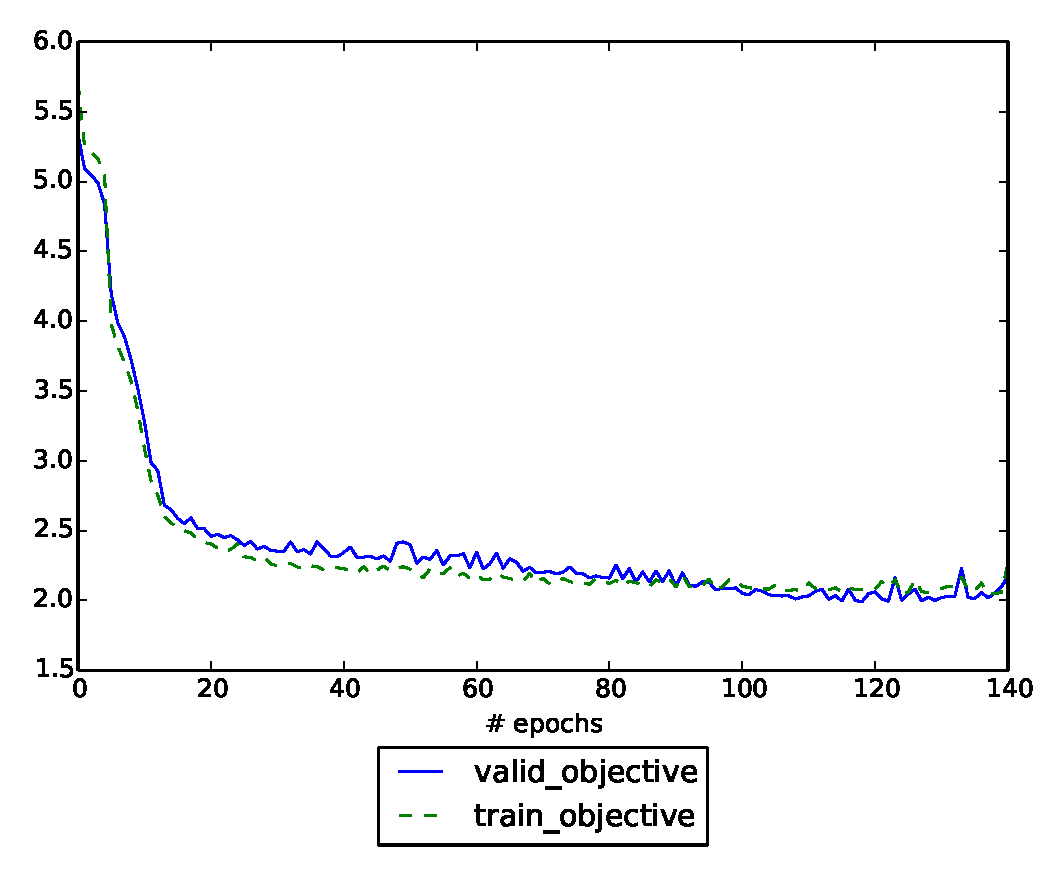
\epsfig{file=images/plot.eps, width=\columnwidth}
\caption{Training curve of the hybrid model with 80 hidden neurons}
\end{figure}

This project used Python and \emph{pandas} for the data analysis, \emph{Pylearn2} \cite{goodfellow2013pylearn2} to construct and test the ANN. The \emph{Forecast} \cite{hyndman2007automatic} R package was used for the ARIMA forecast. 




\subsection{Outlier detection}
\label{sec:outlierDetection}

According to Chebschev's theorem \cite{amidan2005data}, almost all the observations in a data set of system states falls into the interval $[\mu - 3\sigma, \mu+3\sigma]$, where $\mu$ and $\sigma$ are respectively the mean and standard deviation of the data set, and the data points outside this interval are declared outliers. In this paper the ANN is used to predict the gas consumption, for this reason a point will be considered outlier if it will fall outside the $95\%$ confidence interval\footnote{For the following description user \textit{fabee} of \emph{CrossValidated} needs to be mentioned: \url{http://tinyurl.com/l9gvz65}. } expressed for the RMSE. If it is assumed that the difference between the actual values $x_i$ and the predicted value $\hat{x_i}$ have:
\begin{equation}
\hat{x}_{i}-x_{i}	\sim	\mathcal{N}\left(0,\sigma^{2}\right)
\end{equation}
\begin{itemize}
\itemsep0em
  \item mean zero.
  \item follow a Normal distribution (it is assumed that it holds for the large amount of data utilized).
  \item and all have the same standard deviation $\sigma$.
\end{itemize}
\begin{equation}
\label{equation:preRMSE}
\hat{x}_{i}-x_{i}	\sim	\mathcal{N}\left(0,\sigma^{2}\right)
\end{equation}
it is possible to say that \cref{equation:preRMSE} follows a $\chi_{n}^{2}$ distribution with $n$ degrees of freedom. Which means:
\begin{align}
P\left(\chi_{\frac{\alpha}{2},n}^{2}\le\frac{n\mbox{RMSE}^{2}}{\sigma^{2}}\le\chi_{1-\frac{\alpha}{2},n}^{2}\right)	=	1-\alpha\\
\Leftrightarrow P\left(\frac{n\mbox{RMSE}^{2}}{\chi_{1-\frac{\alpha}{2},n}^{2}}\le\sigma^{2}\le\frac{n\mbox{RMSE}^{2}}{\chi_{\frac{\alpha}{2},n}^{2}}\right)	=	1-\alpha\\
\Leftrightarrow P\left(\sqrt{\frac{n}{\chi_{1-\frac{\alpha}{2},n}^{2}}}\mbox{RMSE}\le\sigma\le\sqrt{\frac{n}{\chi_{\frac{\alpha}{2},n}^{2}}}\mbox{RMSE}\right)	=	1-\alpha.
\end{align}
Therefore
\begin{equation}
\left[\sqrt{\frac{n}{\chi_{1-\frac{\alpha}{2},n}^{2}}}\mbox{RMSE},\sqrt{\frac{n}{\chi_{\frac{\alpha}{2},n}^{2}}}\mbox{RMSE}\right]
\end{equation}



\section{Experimental Evaluation}
\label{sec:experimental}
The ANN has been trained with \emph{early stopping}, with a fixed number of training epochs (phases). All the results showed are obtained from a k-fold \emph{Cross-Validation} technique, where the network was trained $k$ times, each time leaving out a subset of data from training in order to test the ANN. The results of the $k$ tests, were divided by $k$. The network was always trained with $70\%$ of the data, $15\%$ was used for validation and the other $15\%$ to test.

Although the Mean Absolute Percentage Error (MAPE) is considered a standard for examining the quality of the models prediction of energy load, it represent an adequate error measure only when the loss function is linear. Recent studies demonstrated it is not \cite{kalogirou2006artificial}\cite{kajl2000evaluation}. Moreover the percentage error is infinite if there are zero values on the series or frequent intermittent data, and it puts a heavier penalty on positive errors than on negative errors \cite{hyndman2006another}. Because of these disadvantages, this paper only considered the minimization of the Root Mean Square Error (RMSE), which penalize large errors. For every experiment the Mean Absolute Error (MAE) was calculated as well. 

\begin{equation}\operatorname{MAPE}\footnote{MAPE errors will be calculated only on the non-zero values, to avoid the problems described before.}=\frac{1}{n}\sum_{i=1}^{n} \frac{|Y_{i} - \hat{Y_i}|}{Y_{i}} \times 100 \end{equation}

\begin{equation}\operatorname{RMSE}=\sqrt{\frac{1}{n}\sum_{i=1}^n(\hat{Y_i} - Y_i)^2}\end{equation}

\begin{equation}\operatorname{MAE}=\frac{1}{n}\sum_{i=1}^n \left| \hat{Y_i}-Y_i\right|\end{equation}

The system was tested with synthetic and measured experiments. The first one refers to author generated data, while the latter used the Ebatech dataset. 




\subsection{Synthetic experiments}
Two days outliers were synthetically generated by different algorithms. In the first one the real consumption was modified by a random value, simulating the system measurement/control malfunction which makes the consumption bouncing up and down (see \cref{equation:synt1}). The second synthetically created day was created adding $50 m^3$ of gas consumption to the real one, creating a pattern which simulates a strange behaviour and/or a malfunction of the heating system (see \cref{equation:synt2}).

\begin{equation}G(t)= G(t)+v*30\label{equation:synt1} \end{equation}
where 
\begin{align*}v \sim \mathcal{N} (0,\sigma^2) \end{align*}

\begin{equation}G'(t)= G'(t)+50\label{equation:synt2} \end{equation}

\begin{figure*}
\centering
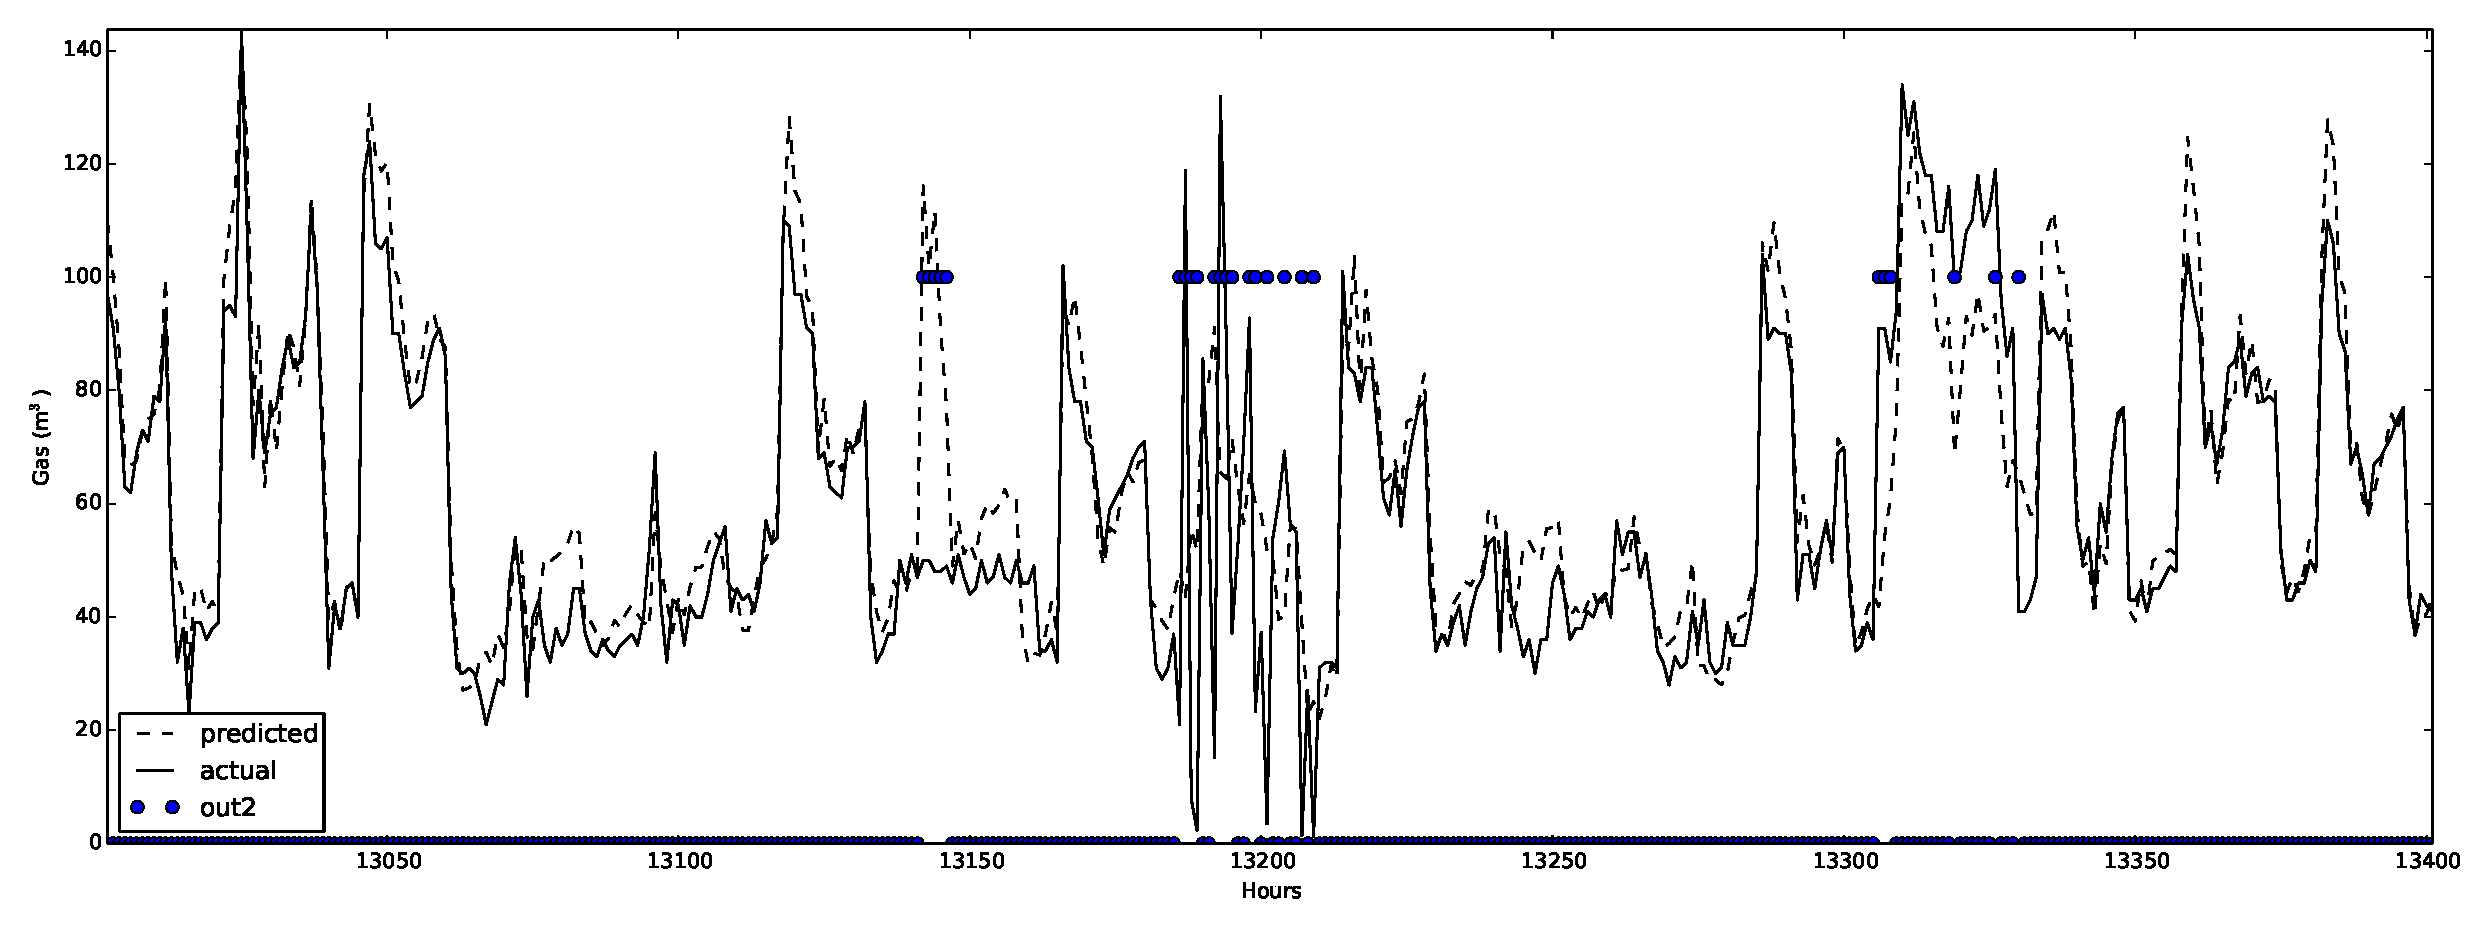
\includegraphics[width=\textwidth]{images/outliersSynt.eps}
\caption{Outlier detection with synthetically generated data. The circle represents the hours where an outlier is detected.}
\label{fig:outlierSynt}
\end{figure*}

The two outliers were correctly detected, as it can be seen in \cref{fig:outlierSynt}.



\subsection{Measured data experiments}
The first test was done by placing a week-end gas consumption in a business day, in order to simulate an anomaly with real data. In \cref{fig:outlierReal} it can be seen that the outlier mechanism works perfectly when the Sunday gas consumption is placed in a weekday. 

\begin{figure*}
\centering
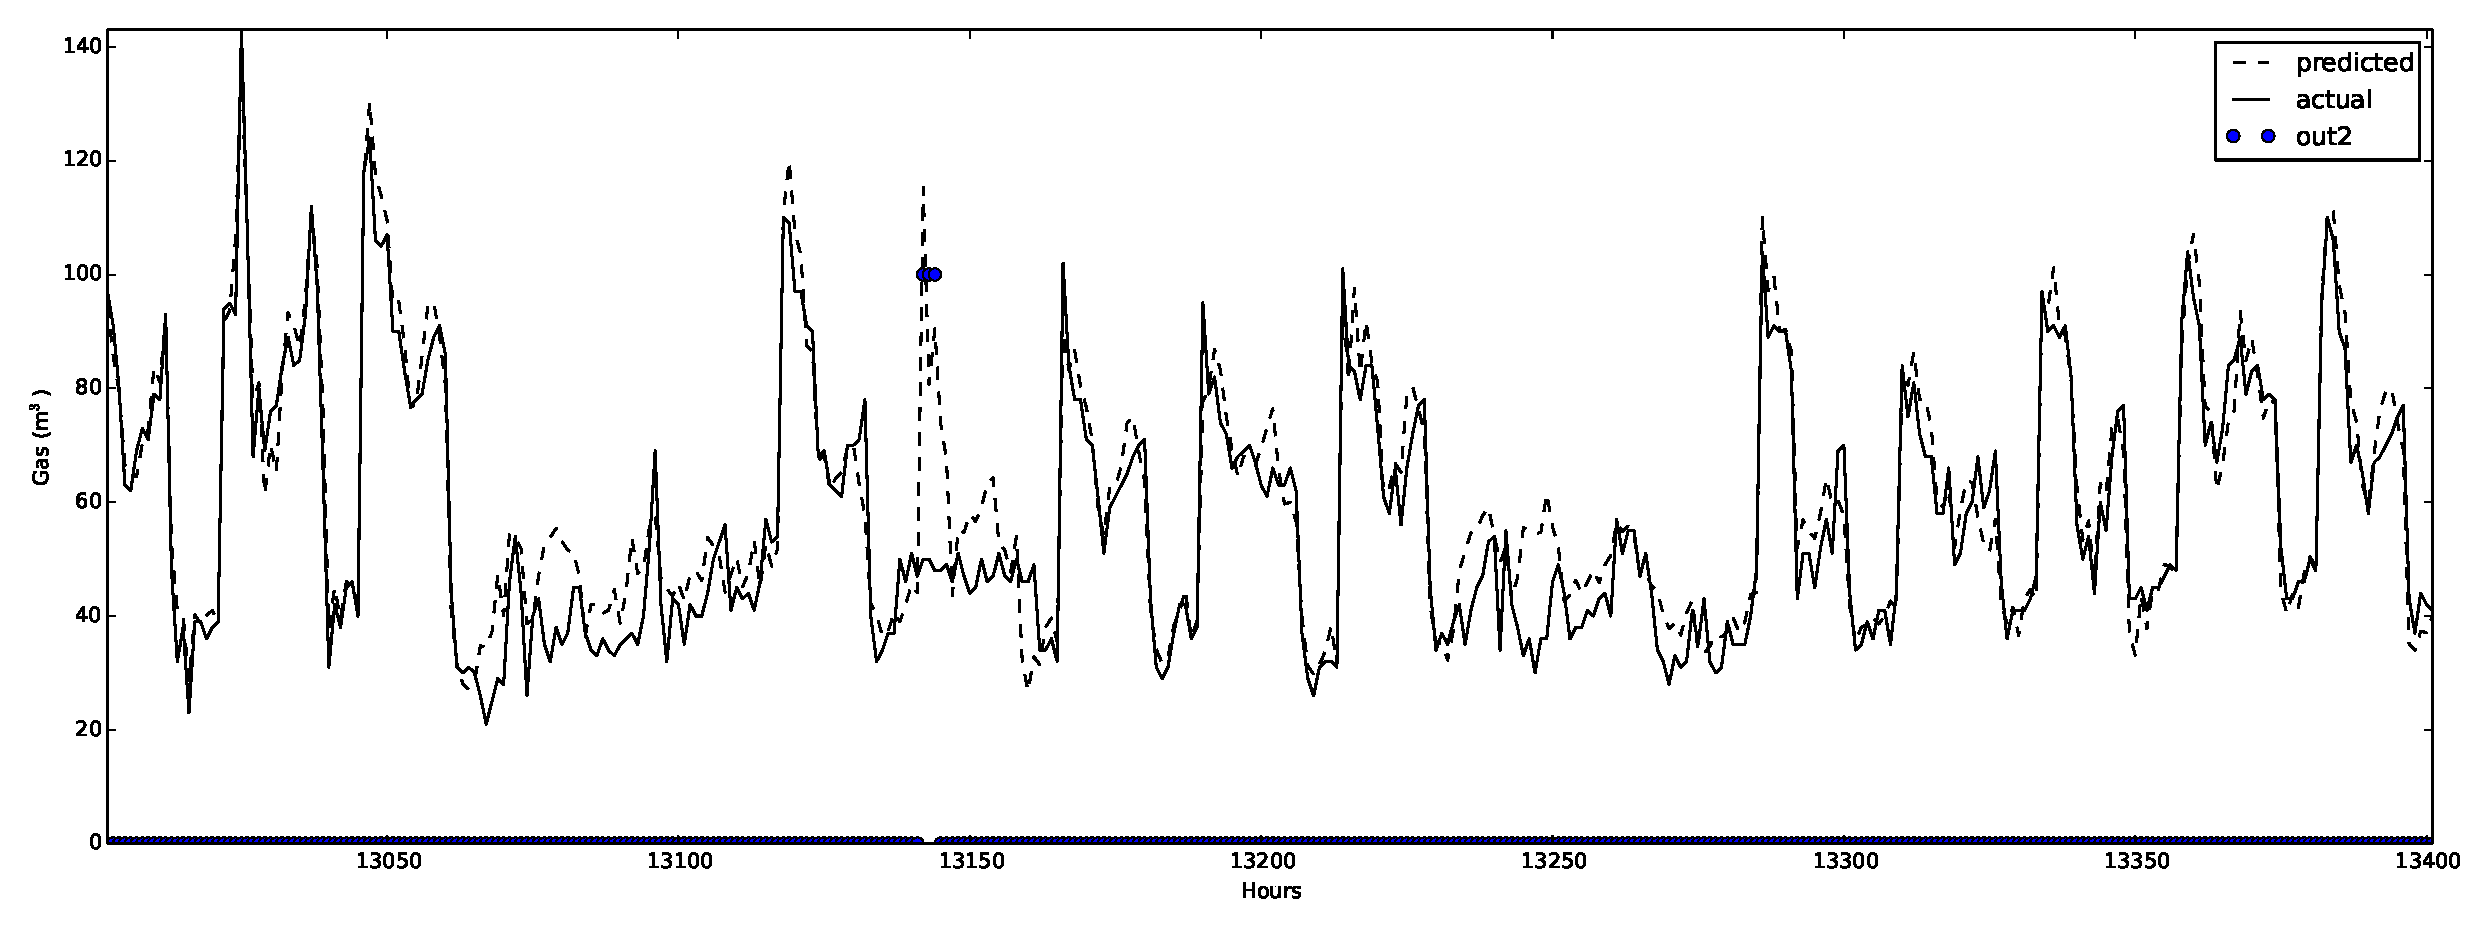
\includegraphics[width=\textwidth]{images/outliersReal.eps}
\caption{Outlier detection where the gas consumption of a weekday was replaced by a Sunday one. The (three) circles represent the outliers detected by the system.}
\label{fig:outlierReal}
\end{figure*}

The outlier was correctly detected, as it can be seen in \cref{fig:outlierReal}. The robustness of the design was proved with different building, listed in \cref{tab:dataset}.

Apart this little experiment, some interesting behaviours were found though this work:
\begin{description}[leftmargin=1pc]
\itemsep0em
  \item[Holidays] Regardless of whenever the school was operational or not, the first tests showed that the Ebatech system was heating the buildings like any other working day. For example Tuesday 25th of December 2012 (Christmas) was heated like a normal business Tuesday even if the building was certainly closed. This causes an avoidable waste.
  \item[Consumption bounces] In \cref{fig:zigzag} a strange zig-zag behaviour can be seen for building 740-NTH. It seems that the system is wasting energy and this shape is totally different from the usual one (\cref{fig:dailyBehaviour}). This lasts for months and it is clear that also the ANN training is affected by this outlier-like behaviour.
\item[Peaks] Around the initial days of September there is a huge bounce of the consumption (up to three times more than the maximal consumption of the year). Is it a test?
In building 761-KMH, irregular peaks during April 2013 were found every day, probably when the heating system turns on.
\item[August with heaters] In building 740-NTH, during August 2009 and August 2011 the heaters were active even without an apparently cold summer.
\item[Outliers] Some other outliers are found but they need to be confirmed by the managers, hopefully after the verification of the previously mentioned behaviours.
\end{description}
All these problems will be immediately reported to the company.

\begin{figure}
\centering
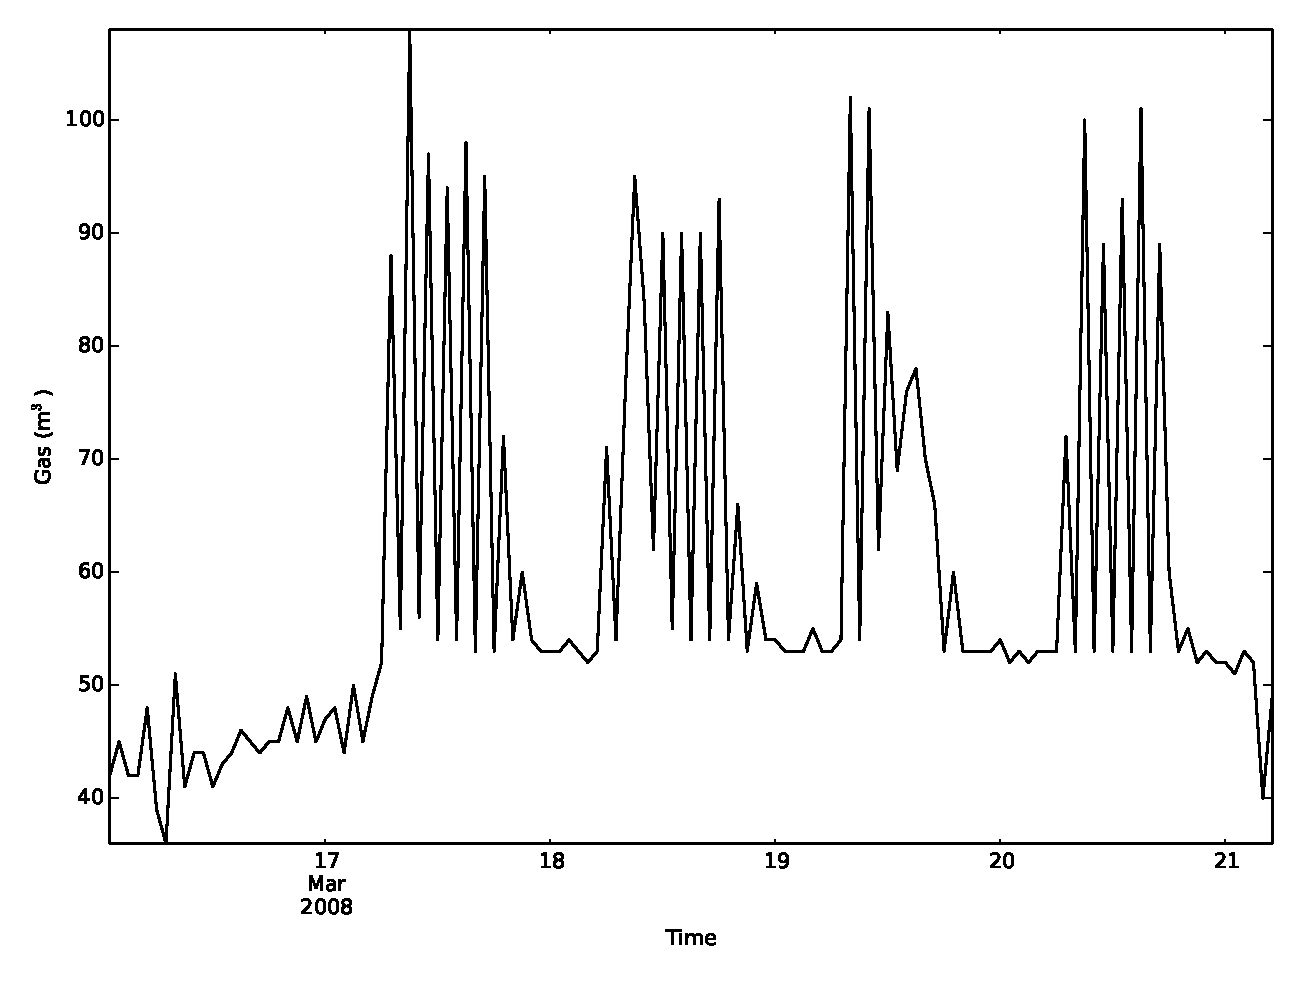
\epsfig{file=images/zigzag.eps, width=\columnwidth}
\caption{Strange zig-zag behaviour found by the algorithm.}
\label{fig:zigzag}
\end{figure}

An ANN with the standard cost function MSE was also trained, apparently resulting in a smaller RMSE error (\cref{tab:ANNresults}). However, the Hybrid MLSE model was more precise, detecting better the possible outliers. They contributed the most to the error.

In \cref{tab:ANNresults2} the results in the different buildings can be read.

\begin{table}
\centering
\begin{tabular}{llllll} \hline
Model     & neurons & epochs & RMSE & MAPE & MAE \\ \hline
ARIMA\tablefootnote{Calculated iteratively as described in \cref{sec:predictor}}      & - & - & 88.50 & 117.27  & 22.52  \\ 
ANN         & 80 & 15 & 11.95 & 34.78  & 8.52 \\ 
HyMSE     & 80 &  70 & 9.4 & 27.66 & 6.90 \\ 
HyMLSE      & 150 & 140 & 10.02 & 30.05 & 7.26 \\ 
\hline
\end{tabular}
\caption{Best selected results in building 740-NTH, to compare the ARIMA, ANN and hybrid model. HyMSE is the Hybrid model with MSE cost function, while HyMLSE is the same model with MLSE cost function.}
\label{tab:ANNresults}
\end{table}

\begin{table}
\centering
\begin{tabular}{llllll} \hline
Model     & neurons & epochs & RMSE & MAPE & MAE \\ \hline
740-NTH      & 150 & 140 & 10.02 & 30.05 & 7.26 \\ 
761-KMH        & 150 & 140 & 2.49 & 18.30 & 1.00 \\ 
\hline
\end{tabular}
\caption{Best selected results for all the buildings.}
\label{tab:ANNresults2}
\end{table}


\section{Future work}
\label{sec:future}

In this project a holidays list was used but the outlier detection can be improved asking a time-table for the buildings, indicating when these are closed.

ARIMA models can't detect more than one seasonality but it can be helped with Fourier terms and ARIMA \emph{dummy variables} to pro­duce rea­son­able fore­casts. When a multi-seasonality is present, a non-parametric model like TBATS\cite{de2011forecasting} could overpass ARIMA and help further the ANN. This recent algorithm is extremely slow, but it is probable that the performance will be improved soon.

ANNs are sensitive to missing values and irregularities, but it was not possible to contact the buildings managers in order to possibly confirm/identify previously known outliers. For this reason the ANN training was done with not entirely clean data, and this probably affected the performance. It is necessary to contact these building managers to further help the training of this algorithm. \\
The features were scaled standardizing them to the range $[-1, 1]$. It is also possible to normalize them to have mean $0$ and standard deviation $1$. In this case Robust estimates of location and scale are desirable if the inputs contain outliers. \cite{iglewicz1983robust} and the recent \cite{mizera2004location} can be the base of a future refine of the ANN inputs.

In a future work it is also possible to analyse the difference between the MSE and the MLSE cost, not only in the prediction, but also in the outlier detection.

Before $2006$, ANNs were almost always associated with the \emph{Backpropagation} algorithm and with the 1-hidden layer architecture. The problem with these architectures is that they get stuck in poor local-optima. In 2006 there was a huge breakthrough, mainly started by \cite{hinton2006fast}, which is called \emph{Deep learning} and it represent the new fashion of ANNs, based on multi hidden layers and new algorithms. Future improvements can be based on Recurrent Neural Networks (RNNs) and Restricted Boltzmann Machines (RBMs) which were recently proved to be interesting in time-series forecasting \cite{busseti2012deep, taylor2009factored, sutskever2013training}.



\section{Conclusion}
\label{sec:conclusion}

Any model can't accurately treat all the situations for a large amount of historical load data. The irregular fluctuation of the gas consumption was hardly predictable, consequently the ANN model was helped with robust cost function and with the well known ARIMA model. Although other papers presented similar models to forecast electric consumption, the hybrid model presented here is almost unique because it focuses on short-term gas consumption forecast, which are very irregular and not easily predictable with classic methods. Since the prediction is very accurate (with RMSE from $8$ $m^3$ in building 740-NTH, to RMSE $2.5$ $m^3$ in building 761-KMH), the outlier mechanism is able to easily detect strange behaviours without the need to possess previous examples of outliers. The scope of this paper was forecasting the highly irregular gas consumption time-series, but it is believed that similar results could be also obtained with the more regular electric consumption time-series. 

It is hoped that this work would lead to new analysis of the energy consumption in public buildings.
%\vfill

%\end{document}  % This is where a 'short' article might terminate


%ACKNOWLEDGMENTS are optional
\section{Acknowledgments}
This internship was economically supported by Universita' degli Studi di Trento. I also thank Jesse Eisses who helped me to find some interesting ideas for this paper.

%
% The following two commands are all you need in the
% initial runs of your .tex file to
% produce the bibliography for the citations in your paper.
\bibliographystyle{abbrv}
\bibliography{sigproc}  % sigproc.bib is the name of the Bibliography in this case
% You must have a proper ".bib" file
%  and remember to run:
% latex bibtex latex latex
% to resolve all references
%
% ACM needs 'a single self-contained file'!
%
%APPENDICES are optional
\appendix
%Appendix A
\section{Sources}
``Very often scientific studies rely on complex textual explanations of what has been done to analyse the data that can overwhelm the reader that has to accept them as an act of faith"\footnote{\url{http://labs.biblioteca.uoc.edu/blog/?p=4332}}. To avoid this, the author provides all the sources\footnote{\url{https://github.com/denadai2/energyUva}}, while the raw data are protected by privacy of the Hogeschool van Amsterdam. The Universiteit van Amsterdam is working to make them available to achieve total reproducibility.

%\balancecolumns

\balancecolumns % GM July 2000
% That's all folks!
\end{document}
